\subsection{The Flat-Sky approximation and Extended Limber Approximation}
The baseline measurement for many cosmic shear studies has focused on the two-point shear correlation function between two tomographic bins $ij$ \citep[for more details see][and references therein]{miraldaescude:1991, kaiser:1992, bartelmann/schneider:2001}, given by
\be
\xi_\pm^{ij}(\theta) = \frac{1}{2\pi}\int \d\ell \,\ell \,P^{ij}_\gamma(\ell) \, J_{0,4}(\ell \theta) \, , 
\label{eqn:xiGG}
\ee
where $J_{0,4} (\ell \theta)$ is the zeroth (for $\xi_+$) or fourth (for $\xi_- $) order Bessel function of the first kind and $P_\gamma(\ell)$ is the shear power spectrum at angular wave number $\ell$ which can be related to the underlying matter power spectrum $P_\delta$, using a Limber approximation \citep{limber:1953} as,
\be 
P^{ij}_\gamma(\ell) = T_l \int_0^{\chi_{\rm H}} \d \chi \, \frac{q_i(\chi)q_j(\chi)}{[f_K(\chi)]^2} \, P_\delta \left( \frac{\nu(\ell)}{f_K(\chi)},\chi \right).
\label{eqn:Pkappa} 
\ee
Here $f_K(\chi)$ is the comoving angular diameter distance out to comoving radial distance $\chi$ and $\chi_{\rm H}$ is the comoving horizon distance.   The lensing efficiency function $q(\chi)$ is given in equation (5) of \citet{hildebrandt/etal:2016}, and the value of $\nu(\ell)$ depends on whether a baseline Limber approximation, $\nu(\ell) = \ell$, or the more accurate extended Limber approximation, $\nu(\ell) = \ell + 0.5$, from \citet{loverde/afshordi:2008} is used.   \citet{kitching/etal:2016} show that the pre-factor $T_\ell$ for the shear power spectrum is given by
\be
T_\ell = \frac{(\ell+2)(\ell+1)\ell(\ell-1)}{(\ell + 0.5)^4} \, .
\label{eqn:Tl}
\ee
The corresponding pre-factor for the convergence power spectrum, along with the pre-factors for a range of other statistics such as the CMB lensing power spectrum and galaxy-galaxy lensing power spectrum, is given in \citet{jk12}.

When a survey is sufficiently small, a flat-sky approximation can be made reducing $T_\ell =1$ and $\nu(\ell) = \ell$.  In \citet{kitching/etal:2016} it is not fully clear which combinations of  $T_\ell$ and $\nu(\ell)$ are considered, so we review them all as summarised in Table~\ref{tab:Tl_nu}, also highlighting which combinations were used in recent cosmic shear analyses.

 \begin{table}[htb]
\begin{center}
\begin{tabular}{ | l | l | c | c  | c |}
\hline
Case & ID & $T_\ell$ & $\nu(\ell)$ & Used in \\ \hline
\citet{kitching/etal:2016} `Standard' & KSt & $1$ & $\ell$ & pre-2014 CFHTLenS papers \\
Baseline Limber `Flat' Sky &  LF & $\ell^4 / (\ell + 0.5)^4$ & $\ell$ & \\
Baseline Limber Spherical & LS & equation~\ref{eqn:Tl} & $\ell$ & \\
Extended Limber `Flat' Sky & ELF & $\ell^4 / (\ell + 0.5)^4$ & $\ell + 0.5$ & \\
Extended Limber Spherical & ELS & equation~\ref{eqn:Tl}& $\ell + 0.5$  & \\
Extended Standard Flat Sky & ESt & $1$ & $\ell + 0.5$ & \citet{joudaki/etal:2016} \&  \\
  &  & & & \citet{hildebrandt/etal:2016}$^*$\\\hline
 \end{tabular}
 \end{center}
 \caption{\label{tab:Tl_nu}Variations on the different approximations that can be made when calculating the shear power spectrum $P_\gamma(\ell)$ (equation~\ref{eqn:Pkappa}), using a Limber approximation.  $^*$We confirm that there is a typographical error in equation 4 of \citet{hildebrandt/etal:2016} which should include the extra term of `$+0.5$' in $\nu(\ell)$ that was incorporated in the cosmological analysis.} 
 \end{table}

Figure~\ref{fig:Cl_xi} shows theoretical models for the shear power spectrum $P_\gamma(\ell)$ (equation~\ref{eqn:Pkappa}), and the shear correlation function (equation~\ref{eqn:xiGG}) for the different variations on the approximations listed in Table~\ref{tab:Tl_nu}.   The Standard and Spherical models agree at the few percent level above $\ell>10$ and below $\theta< 100$ arcmin.  The two outliers are the Baseline and Extended `Flat' Sky Limber cases (LF and ELF) where the \citet{kitching/etal:2016} `Flat' Sky approximation has been made with $T_\ell = \ell^4 / (\ell + 0.5)^4$.    We argue that applying the approximation, that $\ell \pm x \approx \ell$, where $x$ is small, only to the numerator of equation~\ref{eqn:Tl} is inconsistent.    To our knowledge, this form of the flat-sky approximation has not been used in cosmic shear studies to date.

As shown in the lower panels of Figure~\ref{fig:Cl_xi}, the `standard flat' sky approximation used by recent cosmic shear surveys\footnote{The KSt approximation was used for pre-2014 CFHTLenS analysis and the ESt approximation was used for recent CFHTLenS and KiDS analyses}, where $T_\ell = 1$, recovers a very similar result to the spherical sky case.  Over angular scales used in the recent KiDS cosmic shear analysis (where the maximum angular scale $\theta<50.7$ arcmin is shown dashed), these curves differ by less than 1\%.  As such the standard flat-sky approximations that have been used will not impact the cosmological analyses of current surveys.
 
 \begin{figure}
 \begin{center}
 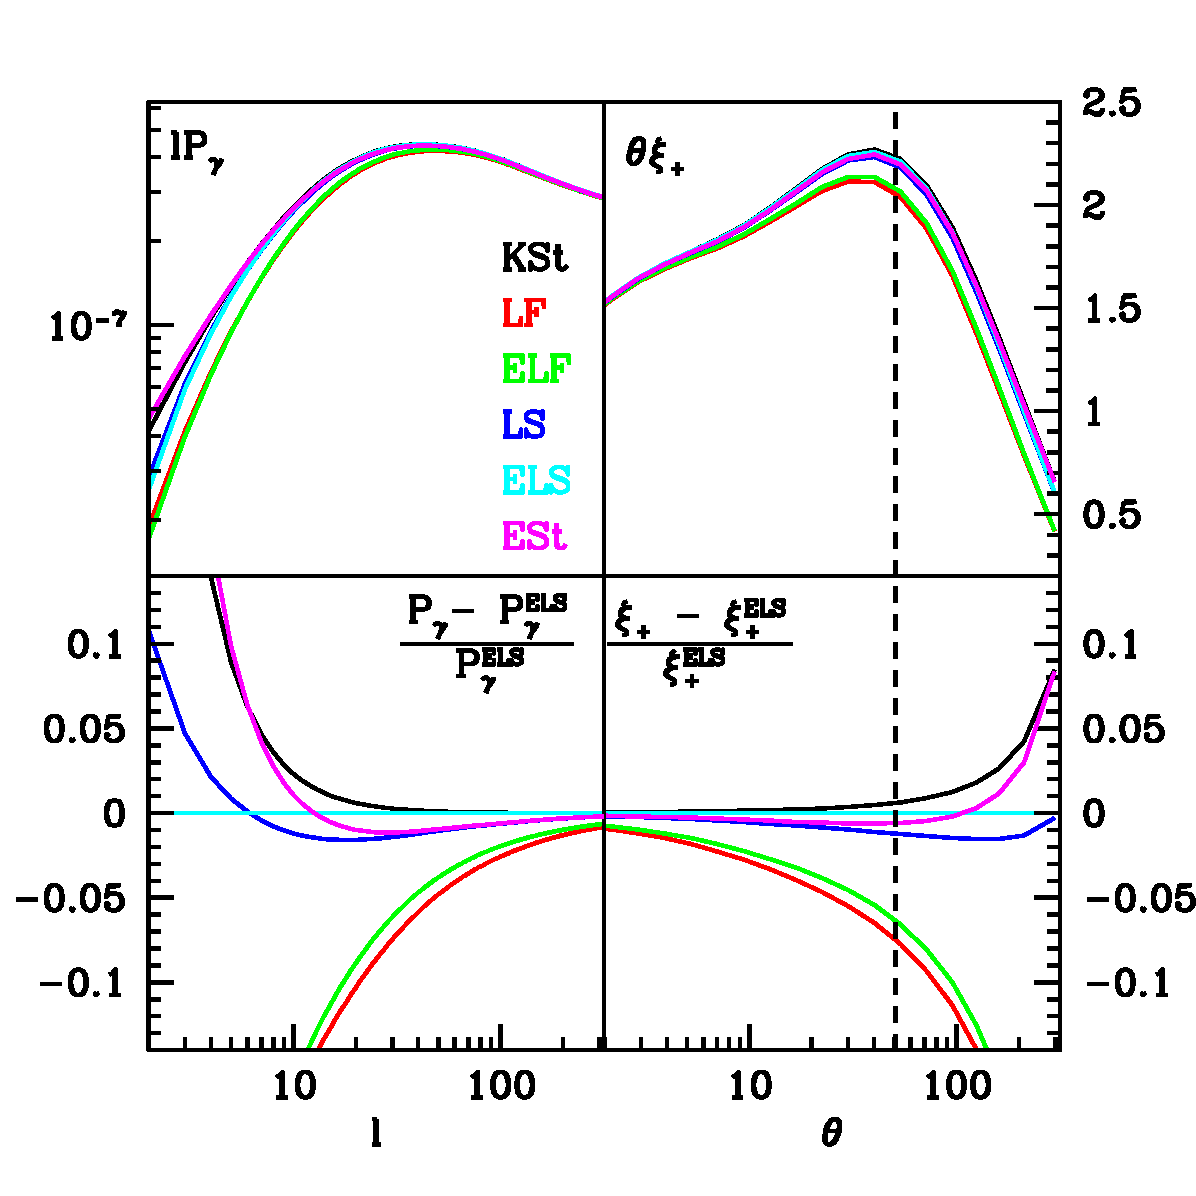
\includegraphics[width=0.85\textwidth]{figures/Cl_xi_comp.pdf}
 \caption{ \label{fig:Cl_xi}\emph{Upper Panels:} Theoretical models for the shear power spectrum (\emph{left}) and shear correlation function $\xi_+$ (\emph{right}) for the different approximations listed in Table~\ref{tab:Tl_nu}, assuming a \citet{planck/cosmo:2015} cosmology and the 2D CFHTLenS redshift distribution. \emph{Lower Panels:} Deviations with respect to the extended Limber spherical sky model (ELS).    The dashed lines in the right panels show the largest angular scale used in the recent KIDS cosmic shear analysis where an Extended Standard (ESt) analysis was used.}
 \end{center}
 \end{figure}
 
 \subsection{Cosmic shear without the Limber Approximation}
In collecting our comments on \citet{kitching/etal:2016} we contacted colleagues who had previously tested the impact of the Limber approximation on cosmic shear studies by comparing a Limber-approximated cosmic shear power spectrum with an exact calculation.  The majority of these analyses, carried out many years ago, remained unpublished in peer reviewed journals as no significant deviation was found\footnote{See for example appendix M of the 2010 PhD thesis from Donghui Jeong (\url{http://www.personal.psu.edu/duj13/dissertation/djeong_diss_appM.pdf}) and Chapter 7 of 2012 PhD thesis from Nicolas Van de Rijt (\url{http://ipht.cea.fr/Docspht/articles/t12/080/public/these_vanderijt2012.pdf}).}.  One notable exception, however, is \citet{giannantonio/etal:2012} who find that for a cosmic shear power spectrum, the extended Limber approximation is consistent with the exact calculation for $\ell>5$, with any differences well within cosmic-variance errors for a Euclid-like survey\footnote{\citet{kitching/etal:2016} comment on this result, but indicate that it is in error owing to the application of a fixed low-$\ell$ limit.  \citet{giannantonio/etal:2012} however state that this limit is only applied in a positive curvature case.}.  We therefore argue that the assertion by \citet{kitching/etal:2016} that the majority of cosmic shear data analyses to date have made an `axiomatic assumption (i.e. an unquestioned and untested assumption at the beginning of the analysis)'  is unwarranted.  Not only is there published work that has questioned and tested the Limber approximation for the cosmic shear power spectrum, individual teams have also verified this result internally for their own cosmic shear analyses.    

Given the insignificant effect of using the Limber approximation found by various groups, the ability to calculate an exact non-Limber solution has unfortunately not been maintained in many theoretical codes over the years.  Instead these codes have evolved to account for (much more) important approximations such as the impact of baryon feedback on the matter power spectrum and non-zero neutrino masses \citep[see for example][]{joudaki/etal:2016, mead/etal:2016}.    Two exceptions to this are recent updates to CLASS \citep{blas/lesgourgues/tram:2011,audren/etal:2013} and CosmicFish \citep{raveri/etal:2016}.  On-going code comparisons have, however, revealed differences that are larger than the expected impact of Limber or non-Limber approximation.   We are therefore unable to readily determine non-Limber theoretical calculations for the shear-correlation function to directly compare with the results of \citet{kitching/etal:2016}.   Instead we refer the reader to Figure 3 of \citet{giannantonio/etal:2012} to draw their own conclusions about the impact of this effect.



 
 
 
 
 
 
 